%\documentclass[10pt]{article}
%\documentclass{sig-alternate}
%\documentclass{llncs}
%\documentclass[twocolumn]{svjour3}
\documentclass[10pt, conference]{IEEEtran}
%\documentclass[10pt, conference, compsocconf]{IEEEtran}
%\documentclass[11pt,draftcls,onecolumn]{IEEEtran}

\usepackage{amsmath}
\usepackage{amssymb}
\usepackage{latexsym}
\usepackage{pifont}
%\usepackage{subfigure}
\usepackage{ifthen}
\usepackage{xspace}
%\usepackage{epic}
%\usepackage{calc}
%\usepackage{verbatim}
%\usepackage{enumerate}
%\usepackage{xspace}
\usepackage{array}
\usepackage{graphicx}
\usepackage{url}
% \usepackage{a4wide}
%\usepackage{extarrows}
\usepackage{color}
\usepackage{booktabs}
\usepackage{bold-extra}
\usepackage{multirow}
%\usepackage{authblk}
%\usepackage{keywords}
%\usepackage{amsthm}
\usepackage{times}
\usepackage{comment}

\renewcommand{\paragraph}{\vspace{3pt}\noindent\textbf}

\newtheorem{Prot}{Protocol}
\newtheorem{Thm}{Theorem}
\newtheorem{Def}{Definition}
\newtheorem{Lem}{Lemma}
\newtheorem{Pro}{Proposition}
% \newtheorem{Ex}{Example}
% \newtheorem{Rem}{Remark}
% \newtheorem{Ass}{Assumption}
% \newtheorem{Cor}[Thm]{Corollary}
% \newtheorem{Conj}[Thm]{Conjecture}
% \newtheorem{Prob}[Thm]{Problem}
% \newtheorem{Sol}[Thm]{Solution}

\newcommand{\Setup}{\textsf{\textup{Setup}}}
\newcommand{\Enc}{\textsf{\textup{Enc}}}
\newcommand{\Dec}{\textsf{\textup{Dec}}}

%\bibliographystyle{plain}
%\pagestyle{plain}
\bibliographystyle{IEEEtran}

%--------------------------------------------------------------------

\begin{document}

\title{Cryptographic Resource Accounting for Decentralized Clouds}

\maketitle

%\begin{abstract}
 This is abstract...
\end{abstract}
       
\section{Introduction} \label{sect:intro}

The concept of cloud computing~\cite{AFG+10}, in large part, is already a reality today.
Computing power is typically {\em centrally} generated in large data centers owned and monopolized by only a few large organizations, e.g., Amazon, Microsoft, and Rackspace, and made available to users via a distributed network.
Centralized clouds may be easier to manage; they are, however, costly to maintain.
Moreover, they may have difficulty in keeping pace with today's and future data growth.
They may also be bandwidth bottlenecks for applications requiring substantial scalability and elasticity~\cite{symform-slide,techrepublic}.

{\em Decentralized clouds} are emerging as attractive alternatives in recent years.
Instead of relying on large and centralized data centers, users harvest the excess computing resources available from Internet-connected computers distributed across the world; in return, the owners of the involved computers earn credits or money (typically in the form of digital currency) proportionate to their contributions.
A few notable examples of such commercial decentralized clouds are Storj~\cite{Storj}, Symform~\cite{Symform}, and MaidSafe~\cite{MaidSafe}.
We note that a decentralized cloud is beyond a multi-cloud, which combines existing centralized clouds into a single virtual cloud storage (e.g., MultCloud~\cite{MultCloud} and Syndicate~\cite{Syndicate}), or a hybrid-cloud, which typically refers to a combination of public and private clouds.
The basic idea of a decentralized cloud here is essentially the same as that of what was traditionally known as volunteer computing, e.g., SETI@home~\cite{Seti@home} and Folding@home~\cite{Folding@home}, or desktop grids~\cite{CKB+07}, e.g., SZTAKI Desktop Grid~\cite{sztaki} and EDGeS~\cite{edges}.
However, a decentralized cloud typically relies on a pricing model, e.g., pay per usage, and the associated accounting and billing services, analogous to those for the existing centralized clouds.
(See~\cite{DP12,MKK13} for further examples and discussions on centralized vs.\ decentralized clouds, and volunteer vs.\ cloud computing.)

- resource usage and billing are top concerns for the majority of IT managers and CIOs 

- existing resource accounting, hard to verify the accuracy and correctness. Also, existing resource metering tools are designed for servers and data centers~\cite{?}.

- The concept of verifiable resource accounting (VRA) was first formalized by Sekar and Maniatis~\cite{SM11}.

- They highlighted that trusted computing can be used to address resource accounting guarantees. However, this cannot be achieved using existing deployed mechanisms. Ideally, a new resource accounting OS or hypervisor should be developed. However, this is not viable given the existing legacy of deployed infrastructure. So, as shown in their subsequent work~\cite{CMP+13}, the only option is to build another layer of lightweight hypervisor on top of existing legacy hypervisors. Nevertheless, there are other challenges remain. For example, such a software-based solution currently can only monitor CPU usage and memory utilization. Also, there's a privacy issue with respect to the cloud provider. It's not clear how the provider's privacy can be protected in terms of their logic and policy of resource allocation (which is usually proprietary).

- the authors acknowledged that what can be done with current TPM technology is only a first step towards an overaching vision. So it may take years to see any deployable and satisfactory TPM-based solution for VRA.

- moreover, it seems infeasible to assume or require each distributed computer in a decentralized cloud model to be equipped with TPM

\paragraph{Goal \& Approach.}
- cryptographic VRA solution can be an appealing immediate and cheaper alternative. In fact, an important point to note is that a cryptographic solution can achieve properties not achievable via TPM, and vice versa. For example, we can provide proofs-of-data-fetch, proofs-of-storage, proofs-of-retrievability, proofs-of-computation, etc., while a TPM-based solution can measure CPU usage and memory utilization. So both approaches can co-exist and complement each other.


\paragraph{Results.}



\section{Problem \& Solution} \label{sect:overview}

\subsection{Problem Definition} \label{sect:problem}

We consider a data owner (client) storing her data in encrypted form on a server, possibly residing on a centralized cloud or a peer-to-peer (P2P) network.
The owner may run computational intensive tasks over the encrypted data.
Instead of performing tasks on the server itself, the owner delegates them to multiple workers residing on a decentralized cloud. 
Each worker fetches its portion of the required dataset from the server, performs the requested computation, and returns the results to the server.
The owner can then, at her discretion, download and verify the results.
The worker is financially rewarded if the verification of the returned results passes through.
This is illustrated in Figure~\ref{fig:model}.
In this work, we ask the question of {\em how can the owner securely and efficiently verify the resource consumption of each worker without relying on a trusted third party or any trusted hardware component}?

\begin{figure}[h!]\centering
  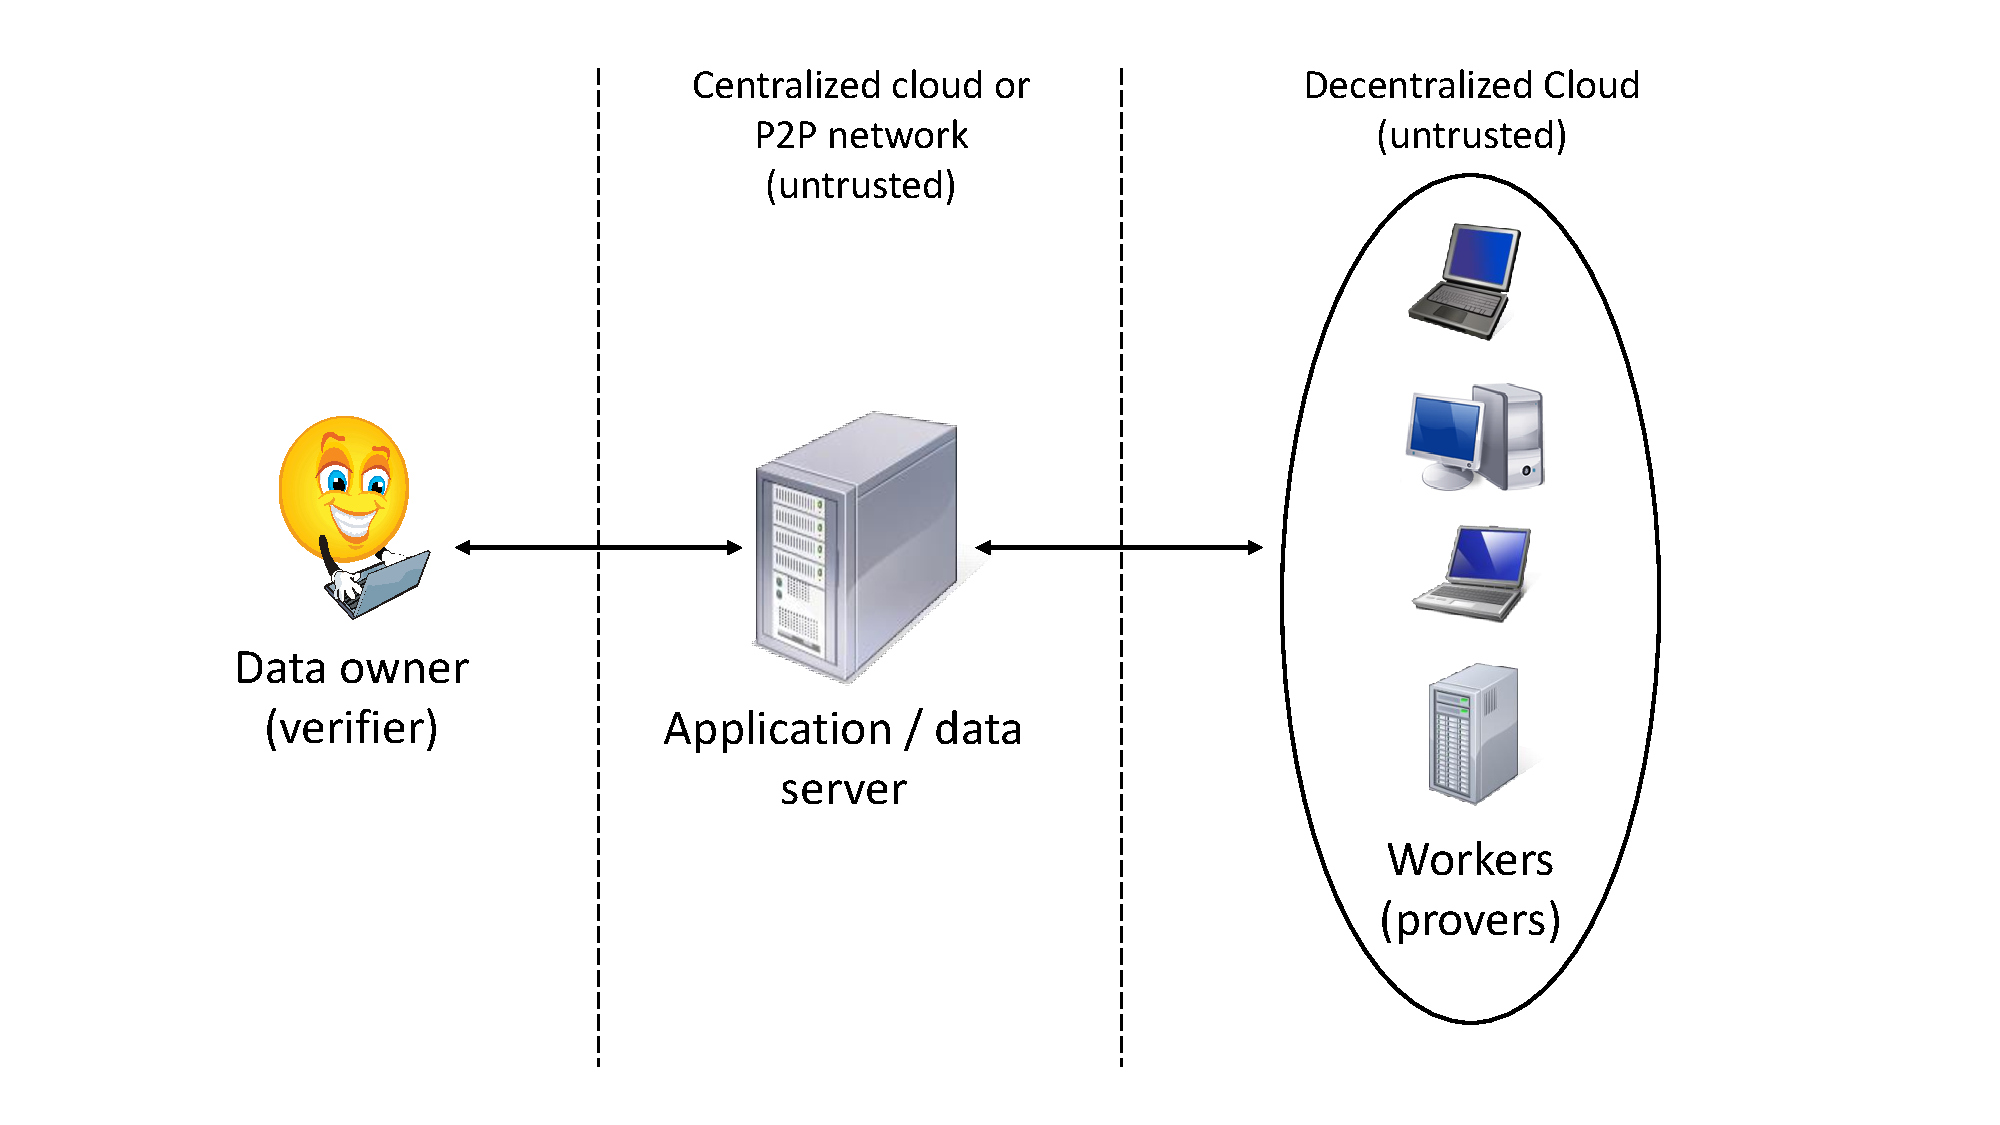
\includegraphics[scale=0.30]{model.pdf}
  \caption{Outsource of data and computation to a decentralized cloud.}
  \label{fig:model}
\end{figure}

Our decentralized cloud setting has the following distinctive characteristics in comparison to centralized cloud settings previously considered:
\begin{itemize}
 \item A data owner distributes her datasets and delegate computational tasks to a decentralized and heterogeneous computing environment.
 \item There exists an intermediate party, i.e., application/data server, which facilitates delegation and distribution of datasets and computational tasks.
 \item The owner can dynamically update her datasets stored on the server, but the data delegated to workers is assumed to be static.
 \item The owner's dataset is stored on the server over an extended period of time, but any data distributed to the worker is only temporarily stored and deleted upon the completion of the assigned task.
\end{itemize}

We note that the introduction of a centralized entity to facilitate distribution of tasks is necessary in our decentralized infrastructure.
In fact, BOINC~\cite{And04} also relies on centralized data and application servers to distribute tasks within a volunteer computing network, and BitTorrent~\cite{Coh03} uses a trusted, centralized tracker to coordinate activities within a P2P network.

\paragraph{Threat Model.}
However, each worker is assumed to be untrusted and they may deviate from the intended computation for various reasons, e.g., to save on computational cost. 
%It is essential, therefore, for the client to be able to verify the correctness of the computation. 
On the other hand, the worker may not trust the data owner either, in the sense that the worker may not be rewarded even if it has completed the computation and proved the correctness of the computation.


\subsection{Challenges} \label{sect:challenges}

\paragraph{Proofs of Data Fetch.}
- One challenge is how to reduce the number of verifications required over multiple workers (currently a prover can convince a verifier with a constant number of challenges/responses for each file). 

- Another issue is that if the worker knows in advance the positions of the challenge data blocks, then it simply downloads only those blocks. Existing POR systems do not encounter such a problem because a file is stored for a relatively extended period of time and different challenges on different positions may be issued to the worker. This forces the worker to download the entire file.

- During update of elements of the dataset, how can the owner update her local state information (used for verifying resource consumption) in an efficient manner?

\paragraph{Proofs of Computation.}
- why POC is sufficient for some applications compared to checking the correctness of computation? (However, for some applications, it may be easier to verify the correctness of computation, which could imply both PDF and POC.)

\paragraph{Fairness.}



\subsection{Solution Overview} \label{sect:solution}


\section{Proofs of Storage} \label{sect:pos}

We adopt Juels and Kaliski's proof-of-retrievability (POR) scheme~\cite{JK07}.
However, we do not require a full-fledged POR scheme for our purposes.
Our setting has the following distinctive characteristics in comparison to those previous POR schemes:
\begin{itemize}
 \item Distributed storage
 \item Asynchronous proof generation: A POS can be generated by each worker individually without being dependent on other workers.
 \item Static \& dynamic data: The owner can dynamically update its datasets stored on the server, but the data delegated to workers is static.
 \item Untrusted data owner and workers: The data owner may refuse to accept a correctly generated POS from an honest worker.
\end{itemize}

- we don't need retrievability, i.e., erasure code

- malicious worker may refuse to release computed results (we discuss how to deal with this problem in \S~\ref{sect:fairness})

- we need to use an encryption scheme which supports secure computation over encrypted data

- one challenge is how to reduce the number of verification required over multiple workers (currently a prover can convince a verifier with a constant number of challenges/responses for each file).

\subsection{Definition} \label{sect:pos-definition}

A proof-of-storage (POS) scheme consists of the following algorithms:
\begin{itemize}
\item \Setup($\lambda$) $\rightarrow k$: The key generation algorithm takes as input a security parameter $\lambda$ and outputs a secret key $k$.

\item \Challenge($k, m$) $\rightarrow V$: The encryption algorithm takes as input a secret key $k$ and a message $m$, and outputs the corresponding ciphertext $V$.

\item \Response($k, V$) $\rightarrow m$: The decryption algorithm takes as input a ciphertext $V$ and a secret key $k$, and outputs the corresponding message $m$ if the key $k$ is correct.

\item \Verify($k, V$) $\rightarrow m$: The decryption algorithm takes as input a ciphertext $V$ and a secret key $k$, and outputs the corresponding message $m$ if the key $k$ is correct.
\end{itemize}


\subsection{Construction} \label{sect:pos-construction}

\begin{figure*}[htb]\centering
  \begin{tabular}{|l|}
    \hline 
    \parbox{0.95\textwidth}{
    \begin{itemize}[leftmargin=*]
    \item \Setup($\lambda$) $\rightarrow k$: The key generation algorithm takes as input a security parameter $\lambda$ and outputs a secret key $k$.

    \item \Challenge($k, m$) $\rightarrow V$: The encryption algorithm takes as input a secret key $k$ and a message $m$, and outputs the corresponding ciphertext $V$.

    \item \Response($k, V$) $\rightarrow m$: The decryption algorithm takes as input a ciphertext $V$ and a secret key $k$, and outputs the corresponding message $m$ if the key $k$ is correct.

    \item \Verify($k, V$) $\rightarrow m$: The decryption algorithm takes as input a ciphertext $V$ and a secret key $k$, and outputs the corresponding message $m$ if the key $k$ is correct.
  \end{itemize}} \\
  \hline
  \end{tabular}
  \caption{A POS scheme.}
  \label{fig:pos}
\end{figure*}
   
We use a POS scheme as specified in Figure~\ref{fig:pos}.

\subsection{Security} \label{sect:security}
\section{Proofs of Computation} \label{sect:poc}

- can we combine proofs of computational effort and random spot checks?


\subsection{Definitions} \label{sect:poc-definition}

\begin{itemize}
\item \Setup($D$) $\rightarrow (\tau,\tau_1,\dotsc,\tau_n)$: The algorithm takes as input a dataset $D$, and outputs a digest $\tau_i$ for each data blocks $D_i$ and a digest $\tau$ for the entire dataset $D$.

\item \Prove($D_i$) $\rightarrow \tau_i$: The algorithm takes as input a data segment $D_i$ and outputs the corresponding digest $\tau)i$.

\item \Aggregate($\tau_1,\dotsc,\tau_n$) $\rightarrow \tau'$: The algorithm takes as input the digests $\tau_i$ corresponding to their respective data segments $D_i$ and outputs an aggregate digest $\tau'$.

\item \Verify($\tau, \tau'$) $\rightarrow \{0,1\}$: The algorithm takes as input the original digest $\tau$ for $D$ and an aggregate digest $\tau'$. It outputs `1' if $\tau=\tau'$, or `0' otherwise.
\end{itemize}

\section{Fairness} \label{sect:fairness}
\section{Evaluation} \label{sect:evaluation}

\subsection{Implementation} \label{sect:implementation}


\subsection{Experimental Results} \label{sect:experiments}
%\section{Conclusions} \label{sect:conclusion}
%\bibliographystyle{abbrv}
\bibliography{IEEEabrv,vc}
%\appendix
%\input{sec-proof}

\end{document}
